\NeedsTeXFormat{LaTeX2e}[2005/12/01]
%%    2010/04/06 v1.0 Vorlage Master-Forschungspraktikum Versuchsauswertung
%%    based on the 2009/10/14 v0.1 GAUBM template by Prof Pruschke

\documentclass[twoside,        %% zweiseitiges Layout
               BCOR12mm,       %% Bindekorrektur 12 mm
% please comment out if report is in English
               english,ngerman, %% Dokumentspr. Deutsch, Alternativspr. Englisch
% please remove comment if report is in English 
%               ngerman,english, %% Dokumentspr. Englisch, Alternativspr. Deutsch
               fleqn,headsepline=false,footsepline=false
              ]{MFPREPORT}

%% Pakete und Definitionen ausgelagert
\usepackage{a4}
\usepackage{multicol}

% language option set in JGNSUM class
\usepackage{babel}
\usepackage{hyperref}

%% FONT:
%\usepackage{lmodern}
\usepackage{times} % sieht besser aus als lmodern
%\usepackage{palatino} % sieht schlechter aus als times
%\usepackage{mathpazo} % very ugly font, to be loaded later ???
%\usepackage{cmbright} % doesn't work either
\usepackage[T1]{fontenc}
\usepackage{textcomp}

\usepackage{ucs}
\usepackage[utf8x]{inputenc}

\usepackage{amsfonts}
\usepackage{amstext}
\usepackage{amsmath}
\usepackage{amsthm}
\usepackage{amssymb}
\usepackage{amsbsy}   % AMS-Boldsymbol

% \usepackage{mathabx} % e.g. for \Sun
%% but not a standard package (neither texlive nor Miktex)
%% so use wasysym (\astrosun) instead
\usepackage{wasysym} % e.g. for \astrosun or \CheckedBox

\usepackage{bbm,mathrsfs}

\usepackage{textcomp} % noch einige coole symbole

\usepackage{sectsty}
\allsectionsfont{\raggedright}

\usepackage[numbers]{natbib}
\citestyle{dinat}
\bibliographystyle{dinat}

\usepackage{makeidx}

\usepackage{url}	% für hübsche URLs mit Link
\usepackage{color}	% für farben a la \definecolor{Gray}{gray}{0.5}
\usepackage{verbatim}
\usepackage{subfigure}
\usepackage{listings}

\usepackage{fancybox}
%usage:
%\begin{Verbatim}[frame=single,label=Titel]
%Verbatim Zeile
%\end{Verbatim}


 \setlength{\textwidth}{16.2cm}
 \setlength{\textheight}{24cm}
 \setlength{\oddsidemargin}{0cm}
 \setlength{\evensidemargin}{-0.5cm}

 %unbedingt nach abmessungen einfügen!
 \usepackage{fancyhdr}
 \pagestyle{fancy}
 %\sloppy % für weniger absatzfehler

 \setcounter{tocdepth}{2}
 \setcounter{secnumdepth}{2}

 \ifreportelse{\numberwithin{equation}{chapter}}{\numberwithin{equation}{section}}
 \theoremstyle{plain}% default
 \ifreportelse{\newtheorem{thm}{Theorem}[chapter]}{\newtheorem{thm}{Theorem}[section]}

 \newtheorem{satz}{Satz}
 \newtheorem{lem}[thm]{Lemma}
 \newtheorem{prop}[thm]{Proposition}
 \newtheorem{kor}[thm]{Korollar}
 \newtheorem{cor}[thm]{Corollary}

 \theoremstyle{definition}
 \newtheorem{defi}{Definition}

 \def\@proof{%
  \if@englishpreamble{Proof}\else{Beweis}\fi
 }
 \newenvironment{bew}{\begin{proof}[\@proof]}{\end{proof}}



%% einbinden einiger nützlicher Befehle
\newcommand{\iflanggerman}[2]{
 \iflanguage{german}{#1}{
  \iflanguage{ngerman}{#1}{#2}
 }
}

% box around the whole equation, number inclusive
\newcommand{\boxedeqn}[1]{%
  \[\fbox{%
      \addtolength{\linewidth}{-2\fboxsep}%
      \addtolength{\linewidth}{-2\fboxrule}%
      \begin{minipage}{\linewidth}%
      \begin{equation}#1\end{equation}%
      \end{minipage}%
    }\]%
}

\iflanggerman{
 \newcommand{\const}{\mathrm{konst}}
 \newcommand{\Const}{\mathrm{konst.}}
}{
 \newcommand{\const}{\mathrm{const}}
 \newcommand{\Const}{\mathrm{const.}}
}

% von Meier
\newcommand{\nbd}{\nobreakdash-\hspace{0pt}}
% example: $K$\nbd{}Vektorraum
\newcommand*{\transpose}[1]{\prescript{t}{}{#1}}
\newcommand*{\conjugate}[1]{\overline{#1}}
\newcommand*{\abs}[1]{\lvert#1\rvert}
\newcommand*{\Mod}{\mathrm{mod}}
\newcommand{\symdif}{\mathbin\triangle}
\DeclareMathOperator{\Graph}{Graph}
\DeclareMathOperator{\id}{id}
\DeclareMathOperator*{\grad}{grad}
\DeclareMathOperator*{\Div}{div}
\DeclareMathOperator*{\rot}{rot}
\DeclareMathOperator{\sig}{sig}
\DeclareMathOperator{\sgn}{sgn}
\DeclareMathOperator{\diag}{diag}
\DeclareMathOperator{\tr}{tr}
\DeclareMathOperator{\Sp}{Sp}
\DeclareMathOperator{\im}{Im}
\DeclareMathOperator{\re}{Re}

\newcommand{\vcentcolon}{\mathop{:}}



\begin{document}
\LabratoryName{FK.TES}{Tunneleffekt in Supraleitern
}
\ProtocolAuthor{Jan}{Weinreich}{janweinreich286@gmail.com}
\Assistant{Christoph}{Meyer}
\ResearchFocus{Festkörperphysik}
% In der naechsten Version beruecksichtigt
%\Collaborator{Vorname}{Nachname}{email}
\ConductedOn{22}{2}{2017}
\date{\today}
% eines von beiden
\CopyNotWanted
%\CopyWanted

\pagenumbering{roman}
\maketitle

%\begin{otherlanguage}{english}
%\end{otherlanguage}

\tableofcontents

\clearpage
\pagenumbering{arabic}

\section{Einleitung}


In diesem Versuch sollen zwei sehr wichtige physikalische Effekte untersucht werden.
Das ist zum einen der Tunneleffekt und zum anderen der supraleitende Zustand eines Festkörpers.
Ersterer ist sehr interessant da es sich um ein Paradebeispiel eines quantenmechanischen Effektes handelt,
der der Energieerhaltung der klassischen Mechanik widerspricht.
\\
Nicht minder interessant ist die Supraleitung, da hier ein quantenmechanischer Effekt direkt messbare Konsequenzen hat.
Hier liegt nämlich ein makroskopischer Quantenzustand vor, was bedeutet dass das ganze System durch
eine Wellenfunktion beschrieben werden kann. 
In technischer Hinsicht wäre es nicht übertrieben zu sagen, dass eine Supraleitung bei Raumtemperatur so etwas wie der "heilige Gral" der Festkörperphysik wäre, weil sich eine Vielzahl großer Anwendungen ergibt, wie zum Beispiel der verlustfreie Transport elektrischen Stromes.
\\
In diesem Versuch soll nun ein Supraleiter/ Normalleiterkontakt hergestellt und eine in der Theorie hier 
näher beschriebene für den supraleitenden Zustand charakteristische Energielücke
vermessen werden. Dafür muss die hergestellte Probe mittels Helium in den supraleitenden Zustand 
überführt werden, damit die kritische Temperatur $T_{C}$ erreicht wird, ab der das Material in den Zustand übergeht.

\subsection{Kommentar}
In diesem Protokoll werden nicht die Daten des Versuches von Erik Bertok und Jan Weinreich vom 22.2.2017 ausgewertet, sondern die eines uns zugeteilten Versuches.
Der Grund ist, dass die von uns hergestellte Probe zwar nach Untersuchung durch das Mikroskop und mit dem Amperemeter in Ordnung war, sich aber bei der Durchführung einige Unregelmäßigkeiten ergaben.
\\
So konnte beispielsweise nicht einmal eine NL NL Kennlinie aufgenommen werden, da der die Kennlinie stets aus seltsame Art oszillierte.




\section{Theorie}

\subsection{Grundbegriffe}
An dieser Stelle ist es sinnvoll kurz auf
einige immer wieder auftauchende Grundbegriffe der hier untersuchten Physik einzugehen. Für die Definition wurde sich hier, wenn nicht anders gekennzeichnet, orientiert an Festkörperphysik von Gross, Marx.
Außerdem stammen nicht gekennzeichnete Grafiken aus der Praktikumsanleitung.



\paragraph{Die Zustandsdichte $D(E)$} gibt an wie viele Zustände in einem gegebenem Energie $dE$ oder auch Impulsintervall $d p$ liegen.
Abhängig von der Dimension besitzt die Zustandsdichte die Elektronen (Fermionen) eine andere Form. 
In den für uns wichtigen drei Dimensionen ergibt sich:
\begin{align}
D(E) = \sum_{\sigma} \frac{(2m^{*})^{\frac{3}{2}}}{2 \pi^2 \hbar^3} \sqrt{E}
\end{align}
Es muss zudem, wie angedeutet über Spin $\sigma=\lbrace \uparrow, \downarrow \rbrace$ summiert werden.
Wie üblich zieht man zur Beschreibung der Elektronen das Modell der effektiven Masse $m^{*}$ heran und setzt dabei voraus dass sie eine parabolische Dispersionsrelation erfüllen.
\\
\paragraph{Die Fermiverteilung $f_{T,\mu}(E)$} gibt im Falle der Näherung freier nicht wechselwirkender und ausschließlich dem Pauli-Prinzip genügender Spin $\sigma = \frac{1}{2}$ Teilchen die Wahrscheinlichkeit an, dass ein Zustand der Energie $E$ bei einer fixen bestimmten Temperatur $T$ sowie chemischen Potenzial $\mu$ besetzt ist. 
Das Pauli Prinzip besagt, dass nicht zwei Elektronen in allen Quanten-zahlen übereinstimmen dürfen. Ausgehend von dieser Zwangsbedingung findet man durch eine statistische Betrachtung die Verteilungsfunktion:
\begin{align}
f_{T, \mu} (E)={\frac {1}{e^{(E-\mu )/kT}+1}}
\end{align}
Bei $T=0$ ist $f_{T,\mu}(E)=1$ für $E \leq E_{F} \equiv \text{ Fermienergie}$, also alle Zustände besetzt und $f_{T,\mu}(E)=0$ für $E > E_{F} $ kein Zustand besetzt. 
Abhängig von $T$ beobachtet man eine schwache Aufweichung der Fermikante. 
Als \paragraph{Besetzungsdichte $\rho$} bezeichnet man, nun da wir die Zustandsdichte $D(E)$ und die Fermiverteilung definiert haben, deren Produkt dessen Integral die tatsächliche Anzahl an Zustanden $N$ angibt:
\begin{align}
N = \int dN = \int_{0}^{\infty} D(E) f_{T,\mu} (E) dE
\end{align}
 
\subsection{Tunneleffekt}
Ein quantenmechanisches Teilchen ($\equiv$ Welle) ist durch seine Wellenlänge und Energie gekennzeichnet. 
Ein freies Elektron, mit kinetischer Energie $T$ dessen Wellenfunktion ebene Wellen sind, kann natürlich ein konstantes Potenzial $V_{B}$ mit Länge $d$ überwinden falls $T \geq V_{B}$.
Aus Stetigkeitsbedingungen und der Schrödingergleichung erhält man jedoch auch für $T < V_{B}$ eine Transmissionswahrscheinlichkeit ungleich Null
\footnote{Voraussetzung ist weiterhin nach Pauli, dass unbesetzte Zustände vorhanden sind, in die getunnelt werden kann.} .
Die Amplitude, dessen Quadrat nach Born die Aufenthaltswahrscheinlichkeit angibt fällt dann innerhalb der Barriere exponentiell ab und schließt sich stetig an die auf der anderen Seite austretende ebene Welle an.
\\
Nach der Transmission ist zudem die Wellenlänge $\lambda^{\prime}$ die gleiche wie beim Eintritt $\lambda$.
\\
Dass die Wellenlänge der austretenden Welle nicht von der Dicke $d$ abhängt drückt die Energieerhaltung aus,
da für ein freies Teilchen
\begin{align}
E = \frac{h^2}{2 m \lambda^2} = E^{\prime}
\end{align}
gilt.
\\
Jedoch wird die Tunnelwahrscheinlichkeit umso kleiner je größer die Dicke der Tunnelschicht ist.
\\
Diese ist in dem Versuch durch die Dicke $d$ der Aluminiumoxidschicht gegeben die zudem eine später gegebene Breite besitzt.
Dieses ist ein sehr guter Isolator, da es keine freien Zustände im Leitungsband gibt.


\subsection{Cooper Paare}
Das radikal verschiedene Verhalten eines Supraleiters im Vergleich zu einem Ohm'schen Leiter bedeutet, dass hier ein anderer Wechselwirkungsmechanismus vorliegt im Vergleich zu klassischen Leitern.
\\
Im folgenden wird eine mögliche qualitative Erklärung
\footnote{siehe Buckler}
gegeben. 
Für dieses Modell betrachten wir ein positiv geladenes Kristall Gitter, wobei wir als grobe Vereinfachung alle Effekte der Valenzelektronen vernachlässigen.
Wir fassen außerdem die Kristallatome als bewegliche positive Ladungswolken auf.
\\
Tritt nun ein Elektron in den Kristall ein so erzeugt dieses eine Verzerrung des Kristalls.
Dies hat zur Folge, dass sich, mit einiger zeitlicher Verzögerung aufgrund der Trägheit (Masse) der Kerne, in der Nähe des Elektrons eine höhere Konzentration an positiven Landungen befindet. 
\\
Falls nun ein zweites Elektron der Spur des ersten folgt so spürt es die nun induzierte positive Ladung als eine attraktive Wechselwirkung, da das erste Elektron auch ein Stück weit entfernt und damit die Coulomb WW klein ist. Zudem tragen die positiven Ladungen zusätzlich mit einer Abschirmung zur Abschwächung der Elektronenabstoßung bei.
Bei einem Supraleiter sind die dadurch entstehenden Anziehungskräfte groß, dass die Abstoßung vergleichsweise klein ist.
\\
Nun wird also eine Art Gleichgewichtszustund erreicht wenn der Abstand der Elektronen gerade der Kohärenzlänge entspricht. 
Diese interpretiert man dann als die Ausdehnung eines neuen Teilchenzustandes, dem Cooper Paar.
\\
Durch theoretische Betrachtungen konnte Cooper zeigen, dass die Gesamtenergie des erwähntes Zweiteilchenzustandes besonders stabil ist, wenn $p_1 = -p_2$. 
\\
Daher wird dieser Zustand bevorzugt angenommen.
Die früher erwähnte Wechselwirkung der Elektronen, die diesen Zustand stabilisiert, wird über Phononen vermittelt.
Diese sind ebenso wie der neue Zustand Quasiteilchen, weil dieser Zustand nur als ein kollektives Phänomen innerhalb des Kristalls auftritt.
Außerdem muss der Spin der Elektronen einander entgegengesetzt sein, weshalb das Cooperpaar einen Gesamtspin Null hat.
\\
Daher genügen die Cooper Paare nicht der Fermi Statistik, was ermöglicht dass alle Paare einen gesamten makroskopischen Zustand bilden können.
\\
Energetisch gesehen liegt dieser kollektive Zustand in der Nähe der Fermi Energie der ungepaarten Elektronen,
da die anderen Zustände bereits besetzt sind.
\\
Hieraus resultiert ein für die ungepaarten Elektronen verbotener Bereich ('Gap') mit der Breite $2 \Delta$, wobei $\Delta$ die Absenkung der Energie bezeichnet, die durch den Cooperzustand erzielt wird.
Um einen gebundenen Zustand aufzubrechen ist nun gerade eine Energie von $2 \Delta$ notwendig.
\\
Des weiteren wird die Zustandsdichte durch die Wechselwirkung der Phononen so verzerrt, dass es Zustände geringer Energie von den Elektronen angenommen werden, die vormals im Gap lagen. 
Dies führt zu einer Abnahme der Zustandsdichte in der Nähe der Kante und damit zu charakteristischen Maxima sowie unbesetzten Zuständen.
Der erläuterte Verlauf der Zustandsdichte im supraleitenden Zustand ist in Abb. \ref{fig:tunnel1} gezeigt.

\subsection{Tunnelkennlinien}

Im folgenden soll es darum gehen die Bandlücke $\Delta$ und damit indirekt den supraleitenden Zustand zu vermessen, um diesen später mit theoretischen Werten zu vergleichen.
\\
Naheliegend wäre es an dieser Stelle ein optisches Experiment durchzuführen, jedoch ist es in der Praxis leichter einen Tunnelstrom zu vermessen.
Der Aufbau ist dabei immer so, dass zwei Schichten (supra-) leitenden Materials durch eine sehr gut isolierende Oxidschicht ($\equiv $ Tunnelbarriere) getrennt sind. 
Nun kann man durch das Anlegen einer Spannung an die beiden leitenden Schichten einen kleinen Tunnelstrom messen der eine Funktion der angelegten Spannung ist ($\equiv$ kinetische Energie der Tunnelelektronen) sowie der Höhe des Potenzialwalls ($\leftrightsquigarrow$ Dicke $d$ der Oxidschicht) welche im wesentlichen die Tunnelwahrscheinlichkeit bestimmt.
\\
Weil es ein einfaches Referenz ist wird zunächst die Tunnelkennlinie für den NL/NL Kontakt betrachtet, siehe dazu Abb. \ref{fig:tunnel1} a.
Bevor eine Spannung $U$ angelegt wird befindet sich das System im Gleichgewicht, weshalb gleich viele Elektronen in beide Richtungen tunneln.
Mit angelegter Spannung werden die Fermienergien $E_F$ relativ zu einander verschoben um $e \cdot U$, sodass ein Nettostrom von links nach rechts in freie sowie energetisch niedriger liegende Zustände stattfinden kann. 
Da die Verschiebung der Fermikanten und damit die Zahl der potenziell tunnelbaren Zustände direkt proportional ist zur angelegten Spannung $U$, können wir ein ohmsches Verhalten $U= R \cdot I$ für die Kennlinie erwarten (Fig. \ref{fig:tunnel2} a).
Die Temperaturabhängigkeit ist im Regime hoher Temperaturen, weil es dann viele Phononen gibt derart, dass die Leitfähigkeit $\sigma \propto T^{-\frac{3}{2}}$.
\\
Anders verhält es sich bei einem Sandwich aus einem Supraleiter und einem Normalleiter, siehe dazu Fig. \ref{fig:tunnel2} b.
Auffällig ist hier, dass erst an einer charakteristischen Tunnelspannung die genau der Energie des Cooperpaares entspricht, einsetzt. Dies ermöglicht später eine Einschätzung für die Größe der Bandlücke  über $\Delta= e \cdot U_c$. 
\\
Für hohe Stromdichten erkennt man, dass der Verlauf sich wieder den Ohmschen annähert, da für große Elektronengeschwindigkeiten  die Zahl der Cooperpaare abnimmt. Zudem ist die Form der SL/NL Kennlinie auch Temperatur abhängig, denn für $T  \neq 0$ liegt eine leichte Verschmierung der Fermikante im Normalleiter vor und zudem liegen auch manche Elektronen im Supraleiter schon oberhalb der Bandlücke, welche sich zudem verkleinert.
\\
Diese Effekte liegen in der idealisierten dritten Kurve (c) für den absoluten Temperatur Nullpunkt nicht mehr vor.
Dort beobachtet man einen steilen Anstieg weil die freien Zustände sich nun alle an der Kante des Leitungsbandes befinden. 




\begin{figure}
\centering
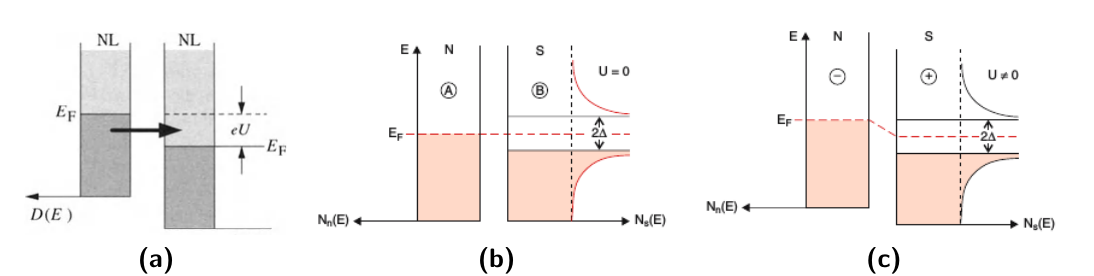
\includegraphics[scale=0.5]{tunnel.png}
\caption{(a) NL-NL, SL-NL wenn keine (b) Spannung angelegt ist und (c) mit Spannung, dies
führt zu einer Verschiebung der Fermikanten um den Wert der angelegten Spannung.}
\label{fig:tunnel1}
\end{figure}

\begin{figure}
\centering
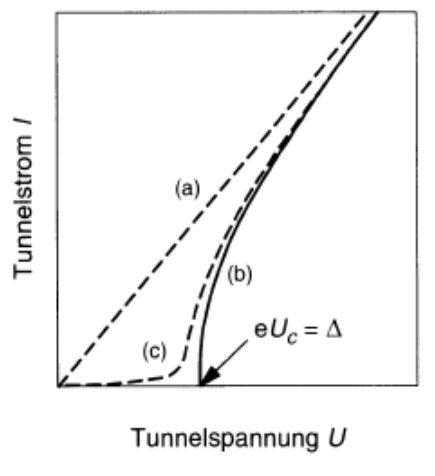
\includegraphics[scale=0.6]{kennlinie.png}
\caption{Verlauf einer NL-SL Kennlinie bei $T=0$ (b), $T \neq 0$ (c), sowie ohmsches
Verhalten eines NL NL Kontakts (a). Beim abs. Temperaturtiefpunkt ist theoretisch der Anstieg
des Tunnelstroms unendlich. Also erwarten wir für kleine Temperaturen größere Werte bei der später
berechneten numerischen Ableitung der Messreihen, siehe dazu Abb. \ref{fig:SLNLDIF}.}
\label{fig:tunnel2}
\end{figure}


\subsection{Vier Punkt Messung}

Dies ist eine Methode bei der die beiden Elektrodenpaar zur Strom und zur Spannungsmessung von einander getrennt sind.
\\
Damit eliminiert man den Leitungs sowie den Kontaktwiderstand bei der Messung, was insbesondere bei der Messung kleiner Tunnelströme von Vorteil ist.

\newpage

\section{Der Versuch}

\subsection{Ablauf des Versuches}


\subsubsection{Herstellung der Probe}

Zunächst muss das Substrat hergestellt werden, das später bei der Messung verwendet wird.
Zu diesem Zweck wird eine Aufdampfanlage verwendet. 
Diese besteht im Wesentlichen aus einer Vakuumglocke in der sich verschiedene über externe Motoren bewegbare Komponenten befinden, wie etwa eine eine Halterung für das (Roh)($\equiv$ Si02) Substat.
\\
Nachdem man das Substat in der dafür vorgesehenen Halterung befestigt mit Aufdampfschablone hat, wird die Kammer mit zwei Vakuumpumpen für verschiedene Druckbereiche evakuiert auf ungefähr $10^{-5} \text{ bar}$, was effizienter ist als nur eine Pumpe einzusetzen.
\\
Nun wird als erstes durch Bedienung der Anlange die eine Goldschicht circa $100 \text{ nm}$ dünne Schicht auf das Substat aufgedampft ($\equiv$ gesputtert).
Die Dicke kann hierbei mit einem Schwingquarz von einer Anzeige abgelesen werden.
Die Anlange kann dann aus der Änderung der Frequenz durch die Ablagerung den gewonnen Trägheitsmoment und daher die Masse der Ablagerungsschicht berechnen.
Zu diesem Zweck muss man zudem noch der Anlage angeben, welches Material aufgedampft wird.
Zuvor wird noch Argon bis auf einen Druck von $10^{-2} \text{ mbar}$ eingelassen und mit einer von der Anlage eingestellten Spannung ionisiert.
\begin{figure}
\centering
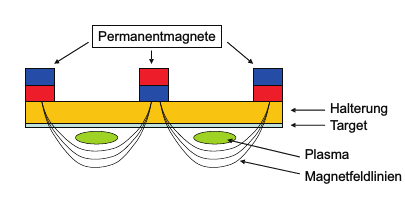
\includegraphics[scale=0.9]{magneton.png}
\caption{Die Anordnung aus Magneten, der Substrathalterung und dem eingeschlossenem Plasma.}
\label{fig:aufbaub}
\end{figure}
Daher können die Argon Ionen nun durch eine Spannung von bis zu $1 \text{ keV}$ die Goldelektrode beschleunigt werden. Das dabei entstehende Plasma wird zusätzlich durch ein Magnetfeld fokussiert.
Die kinetische Energie einiger Ionen reicht dann aus, um einige Goldatome zu lösen welche sich dann aufgrund der Maske an den dafür vorgesehenen Platz des Substrates ablagern.
\\
Als nächstes muss die Aluminiumschicht aufgedampft werden. 
Dazu wird das Substat auf dem schwenkbaren Arm zunächst um $180^{\circ}$ gedreht. 
Nun befindet sich unterhalb des Substrates ein Wolframdraht auf dem man zuvor das Aluminiumpallet gelegt hat.
Der Schmelzdraht besteht aus Wolfram, aufgrund der hohen Hitzebeständigkeit des Materials.
\\
Bevor nun die Schmelzspannung über das Bedienrad der Anlange hochgeregelt wird, muss noch Aluminium als Aufdrampfmaterial ausgewählt werden. Zudem sollte des Hochdrehen nicht zu schnell geschehen, da ein Vorwärmen notwendig ist um die zuvor oxidierte Schicht zu entfernen. Hinzukommt noch dass man eine Schutzwand zwischen dem Aluminium und dem Substat ausfährt und diese erst dann wieder entfernt, wenn das Aluminium geschmolzen ist.
\\
Sobald die Trennwand entfernt ist, beginnt sich die Aluminiumschicht aufzubauen bis man eine Dicke von etwa 50 nm ablesen kann.
\\
Weil das Aluminium oberflächlich oxidiert sein soll wird über ein Belüftungsventil eine wohl dosierte Menge an Luft eingelassen.
Damit beträgt die Dicke der $Al_{2}O_{3}$ Schicht circa 5 nm.
\\
Im Anschluss daran wird wieder gepumpt bis die Bedingungen vor der Belüftung wieder erreicht sind. Nach der gleichen Art wie beim Aluminium wird nun die Bleischicht aufgetragen ($\approx 250 \text{ nm}$).
\\
Interessant ist nun noch die Anmerkung, dass sich die Vakuumglocke dabei zunächst gräulich färbt und anschließend glänzend wird, denn durch das kombinierte freisetzen der Al und PB Schicht hat man im Grund einen Spiegel hergestellt sodass die Vakuumglocke undurchsichtig wird.
Dazu können auch die Bilder des Aufbaues im Anhang betrachtet werden.
\\
Nach diesem Herstellungsprozess müssen insbesondere die Tunnelkontakte genauer untersucht werden. So ergibt sich ein erstes Bild über die Qualität der Probe.
\\
Bei unserer Probe konnten wir keine Unreinheiten finden und auch eine Vermessungen der Kontakte mit einem Amperemeter zeigte, dass alle Kontakte richtig sitzen.
Daher wurde das Substat dann in die dafür vorgesehene Kryostatvorrichtung eingebaut, welche aus einer metallenen Stange besteht an deren Ende man die Probe einspannt.
Zusätzlich muss zur Reduzierung des Kontaktwiderstandes Indium verwendet werden, um eine Verbindung zwischen der Probe und den Kontakten der Stange herzustellen.


\subsection{Messprozess}
In der Praxis sind die Messreihen weitestgehend automatisiert, weil man mit einem bereits existierendem Computerprogramm einfach den zu vermessenden Spannungs oder Strombereich einstellen kann, welcher dann von der Anordnung durchlaufen wird.
\\
In einem ersten Schritt wird nun die NL NL I-U-Kennlinie aufgenommen bei Zimmertemperatur.
\\
Für die Effekte der Supraleitung ist nun eine Abkühlung des Kyrstats notwendig. 
Es erfolgt daher ein 'Vorkühlen' mit flüssigen Stickstoff mit dem allerdings nur ungefähr 77 K erreicht wird. 
Im weiteren Verlauf hat das Stickstoff die Funktion einer isolierenden Atmosphäre zwischen Raumtemperatur und dem Helium.
\begin{figure}
\centering
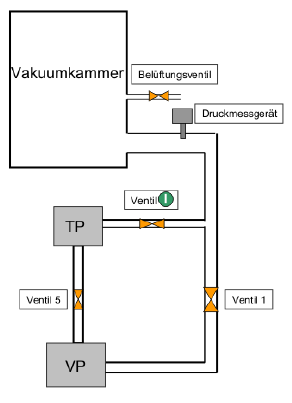
\includegraphics[scale=0.9]{vakuum.png}
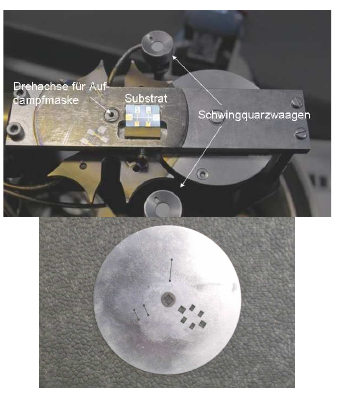
\includegraphics[scale=0.9]{aufbau.png}
\caption{Links:
Die Skizze zeigt schematisch die Verbindungswege der Turbo-(TP) und Vorpumpe  (VP) für die
Vakuumkammer sowie die Position des Druckmessgerätes und des Belüftungsventils in diesem Kreislauf.
Rechts:
Gezeigt sind die Halterungsvorrichtung für die Probe und die Schablone für das Beschichten.
}
\label{fig:aufbau}
\end{figure}
Daher ist es zur Ermittelung der SL-NL Kennlinie erforderlich, dass eine weitere Kühlung mit Helium erfolgt. 
Eine weitere Abkühlung wird über die Dampfdrumerniedrigung des Helium Stickstoffgemisches erreicht.
Dabei wird natürlich nur näherungsweise eine der erwünschten Temperaturen von zum Beispiel 3 oder 2 K erreicht. Dies führt zu Fehlern, die mithilfe der Dampfdruckkurve von Helium 4 (siehe Abb. \ref{fig:dampf} in Diskussion) abgeschätzt werden können.


\subsection{NL-NL Kennlinie}

Wie im Theorieteil angesprochen erwarten wir bei Raumtemperatur das unspektakuläre ohm'sche Verhalten. 
Also einen linearen Zusammenhang zwischen Strom und Spannung.
Da es ohne Spannungsdifferenz keinen Strom gibt verläuft die Gerade zudem durch den Ursprung.
Durch lineare Regression ergibt sich zudem die Möglichkeit den Widerstand oder die Leitfähigkeit des Tunnel-Kontaktes zu berechnen.
\\
Die Steigung ergab einen Wert von $m = (0.00759  \pm 0.000003)  \frac{A}{V}$ für die Leitfähigkeit. Wobei wir für den Strom einen maximalen Fehler von $ \sigma_{I}=0.0001 A$ angenommen haben. 
Der y-Achsenabschnittes ist wie erwartet sehr klein, was auch aus der Abb. \ref{fig:NLNL} in der die Daten ebenso wie der lineare Fit gezeigt sind, deutlich wird.

\begin{align}
R:={\frac UI}={\mathrm {const.}}
\end{align}
Aus der Steigung berechnet sich ein Widerstand von $R=(131.72 \pm 0.05) \Omega$ wobei $\sigma_{\Omega} = \frac{\sigma_{m}}{L} $.
\begin{figure}[h]
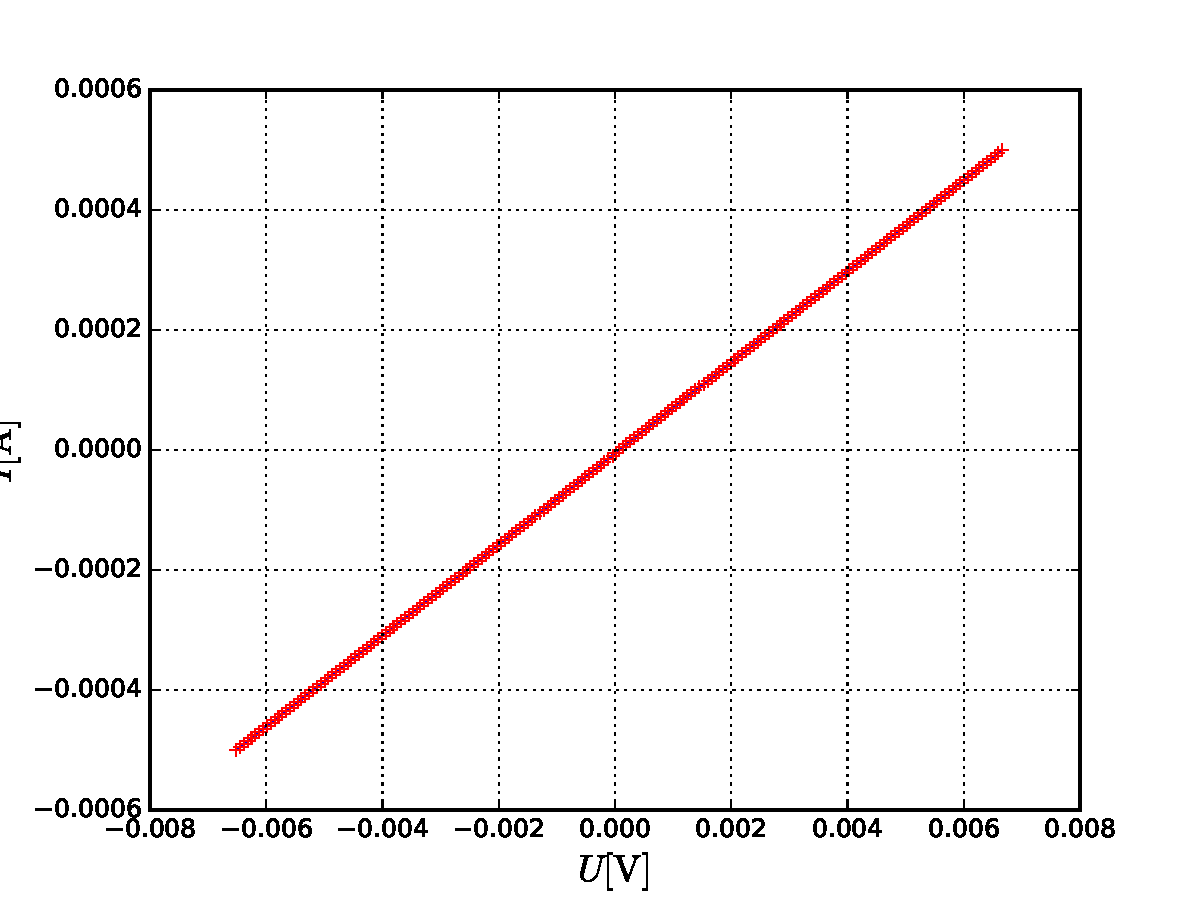
\includegraphics[scale=0.9]{1.pdf}
\caption{NL NL Kennlinie folgt wie erwartet dem Ohmschen Gesetzt.}
\label{fig:NLNL}
\end{figure}
Wie sich andere Tunnelkontakte verhalten bei hohen Temperaturen können wir nicht beurteilen, da uns die entsprechenden Messdaten fehlen.

\subsection{SL-NL Kennlinie}

Als nächstes wurde die U-I Kennlinie des gleichen Kontaktes bei niedrigen Temperaturen vermessen. Zudem ist zum Vergleich der oben diskutierte Verlauf bei Raumtemperatur ($\approx 25^{\circ} C$). In Abb. \ref{fig:SLNL} ist erkennbar, dass der erwähnte Hochtemperaturverlauf in etwa eine asymptotische Grenze für die Verläufe unterhalb der Sprungtemperatur darstellt. Warum dies nicht genau der Fall ist wird in der Diskussion angesprochen.
\begin{figure}
\centering
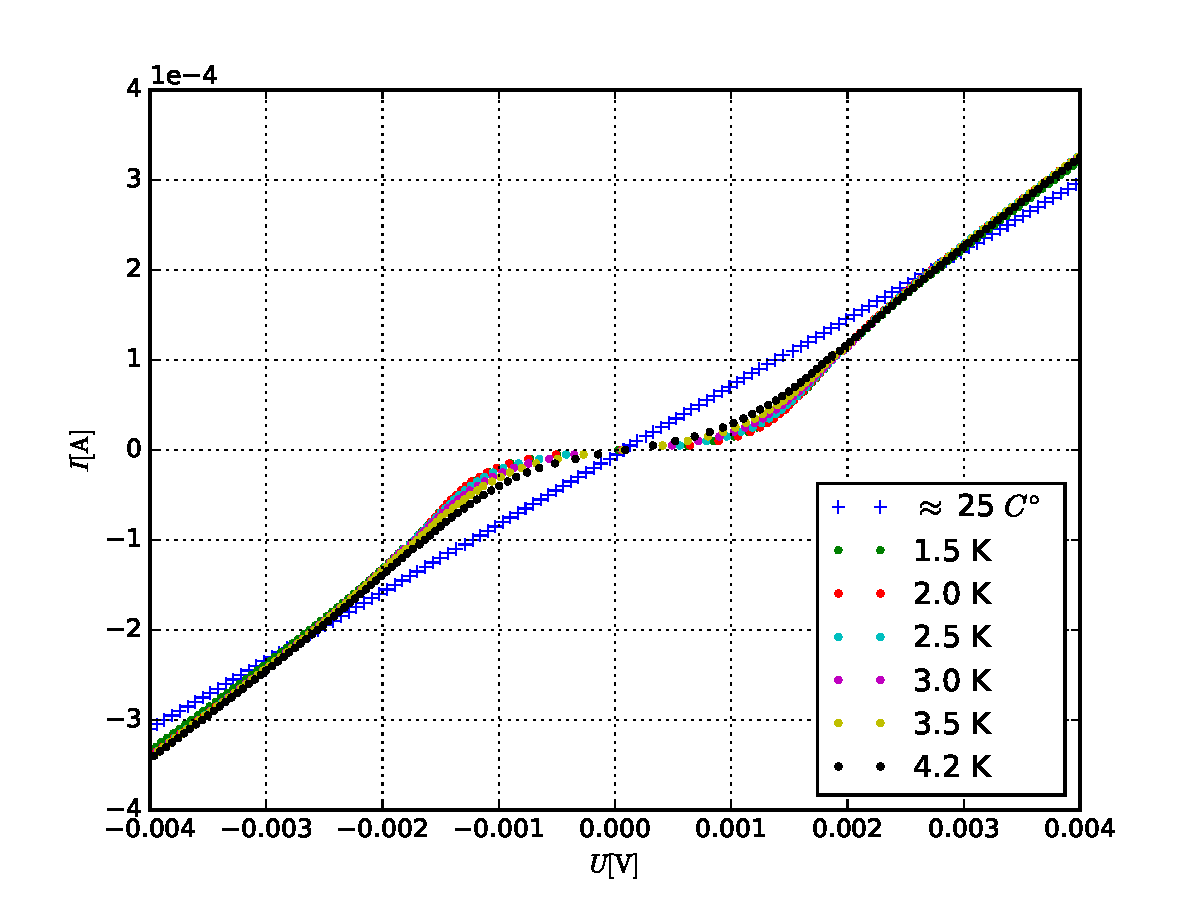
\includegraphics[scale=0.7]{2.pdf}
\caption{Verlauf der SL NL Kennlinie für diverse Temperaturen. Der die Kennlinie bei Raumtemperatur wird bei hohen Tunnelspannungen in etwa angenähert. Charakteristisch für die Supraleitung ist der Sattelpunkt bei $0 V$.}
\label{fig:SLNL}
\end{figure}
\\
Es wurden neben der Raumtemperatur sechs andere Temperaturen untersucht:
\\
$1.5 \text{ K}, 2.0 \text{ K}, 2.5 \text{ K}, 3.0  \text{ K}, 3.5 \text{ K}, 4.2 \text{ K}$.
\\
Es wird aus dem Verlauf des Graphen deutlich, dass zunächst eine gewisse Energiebarriere überwunden werden muss, bis ein Strom fließen kann, wenn eine Temperatur unterhalb von $T_C$ vorliegt.
Der Grund dafür ist, dass zunächst eine charakteristische Energie $2 \Delta$ für das aufbrechen der Cooperpaare aufgebracht werden muss, siehe Abb. \ref{fig:tunnel2}. 
Den nur so können die Elektronen, welche sich noch nicht im gepaarten Zustand vorliegen die Energielücke von $2 \Delta$(siehe Abb.) überwinden \ref{fig:tunnel1}. Dies ist der Grund weshalb beispielsweise in dem Intervall $0-0.001 V$ fast gar kein Strom fließt. 
Zudem beobachtet man, dass der Verlauf in diesem Regime umso flacher ist je niedriger die Temperatur, siehe Abb. \ref{fig:SLNLB} für eine Detailansicht.
Dies entspricht auch den Erwartungen die wir aus der theoretischen Betrachtung gewonnen haben, denn bei $T > 0$ sind bereits manche Zustände oberhalb der Fermikante besetzt und der Verlauf wird etwas verschmiert.

\begin{figure}
\centering
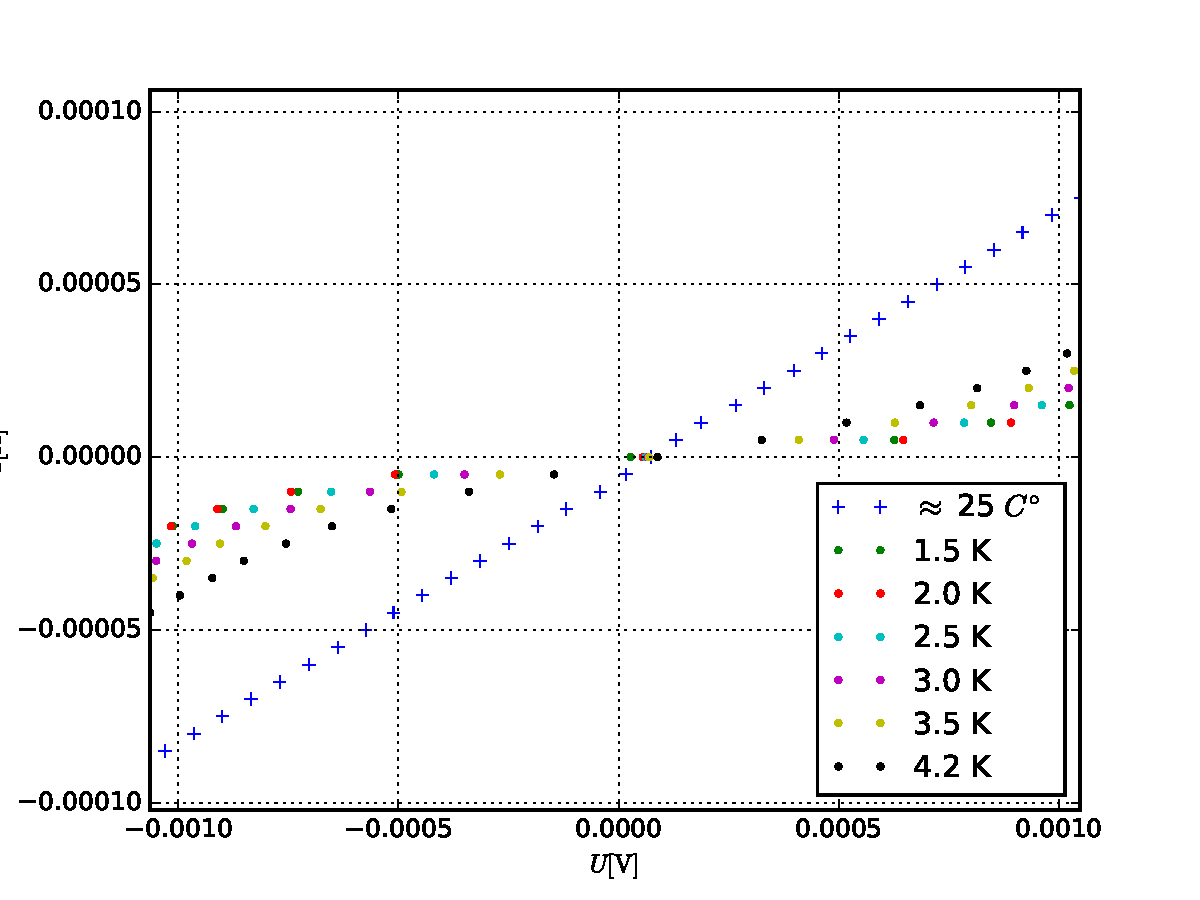
\includegraphics[scale=0.6]{2B.pdf}
\caption{Detailansicht des obigen Verlaufs zur Verdeutlichung der Temperaturabhängkeit.}
\label{fig:SLNLB}
\end{figure}

\subsection{Bestimmung der Energielücke}

Um die Energielücken zu bestimmen muss die Ableitung des gemessenen Verlaufes für den Strom nach der angelegten Spannung berechnet werden.
Zu diesem Zweck wurde numerische Ableitung mittels Python berechnet.
Das Skript verwendet den zentralen Differenzialquotienten
($\equiv$ Mittelwert aus rechtsseitiger und linksseitiger Ableitung) in der diskretisierten Form:
\begin{align}
\frac{d I}{d U} \approx \frac{1}{2} 
\left(
\frac{I_{j+1}-I_{j}}{U_{j+1}-U_{j}} 
+
\frac{I_{j}-I_{j-1}}{U_{j}-U_{j-1}}
\right)
\label{eq:numdiff}
\end{align}
\begin{figure}
\centering
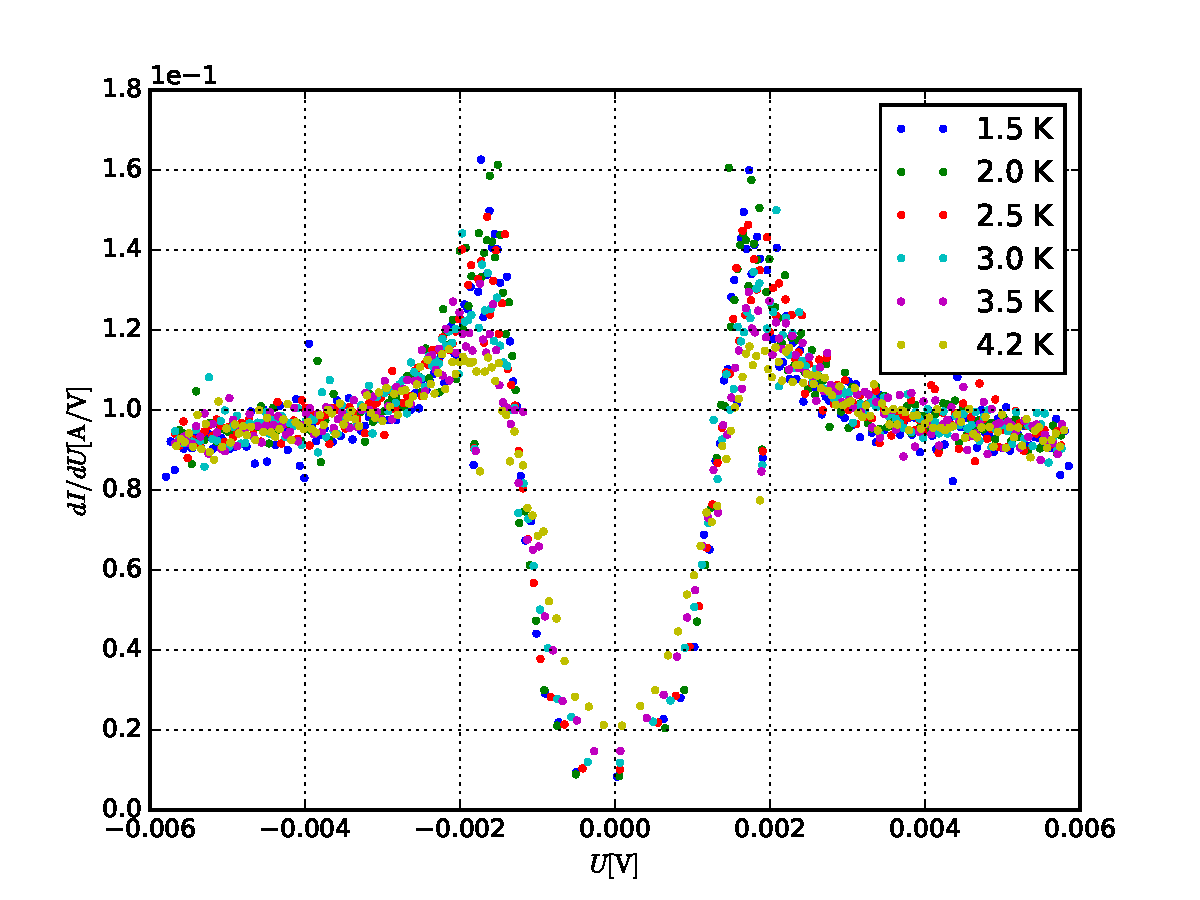
\includegraphics[scale=0.7]{3.pdf}
\caption{Gezeigt sind die numerischen Ableitungen gemäß Gleichung (\ref{eq:numdiff}) der I-U SL NL Kennlinien aus Abb. \ref{fig:SLNLB}. 
		Für die zu bestimmende Breite des Plateaus der Kennlinie sind die hier gut erkennbaren Maxima relevant.}
\label{fig:SLNLDIF}
\end{figure}
Mit dieser Definition der Ableitung ergibt sich der Verlauf in Abb. \ref{fig:SLNLDIF}.
Nun können die Maxima dieses Verlaufes aus den Daten abgelesen werden
und die dazu gehörenden Werte für die Spannung, um den Spannungs
Bereich abschätzen zu können in dem für den supraleitenden Fall näherungsweise noch kein Strom fließt.
Natürlich hätte man an dieser Stelle auch beispielsweise den Mittelwert der Punkte nehmen können die um das gemessene Maximum liegen.
Hierbei ist es aber nicht klar ob dies wirklich zu besseren Werten geführt hätte, denn man müsste sicher des gemessene Maximum einer Messreihe stärker gewichten als die umgebenden Punkte. 
Daher haben wir uns für die einfachere Methode entschieden stets einfach direkt die Maxima mit hinreichend großem Fehler zu nehmen.
\\
Nun ergibt sich so für jede Messreihe einer 
Temperatur ein Wert für die Bandlücken Energie durch
\begin{align}
\Delta \approx \frac{e(U_{rechts}-U_{links})}{2}
\end{align}
Da wir als einfache Schätzung die rechten und linken Maxima jeder Messreihe
als gute Werte angenommen haben wird der Fehler als relativ groß
angenommen.
Dies haben wir für alle Messungen als 1 mV eingeschätzt.
Zudem wird auch noch berücksichtigt, dass sich beim Berechnen der Differenz ein Fehler ergibt.
Der Fehler des rechten ist natürlich auch der des linken Maximums
\begin{align}
\sigma_{\Delta_{\text{Max}}} = \sqrt{\sigma_{\text{Max, right}}^2 + \sigma_{\text{Max, left}}^2} \approx 
1.4 \cdot \sigma_{\text{Max, right}}
\end{align}

\begin{table}[]
\centering
\caption{Erste Spalte zeigt den gemessenen doppelten Wert für die Energielücke,
zweite die zugehörige entdimensionalisierte Größe, es folgen die Werte gemäß Korrekturformel
(\ref{eq:korrformel}) mit temperaturabh. Fehlern gemäß Glg. (\ref{eq:fehlerkor}). }
\label{my-label}
\begin{tabular}{|l|l|l|l|l|}
\hline
Temperatur K & $ 2 \Delta(T)$ in mV  (unkorr.)    & $\frac{2\Delta (T)}{k_{B} T_{C}}$ & $\Delta (T)_{k}$  in mV  (korr.)                              & $\frac{2\Delta (T)}{k_{B} T_{C}}$         \\ \hline
1.5  $\pm$ 0.075        & 3.5 $\pm$ 1.4 & 5.6 $\pm$ 2.3      & 1.55 $\pm$ 1.0  & 5.0 $\pm$ 3.3  \\ \hline
2.0 $\pm$ 0.2         & 3.0 $\pm$ 1.4 & 4.8 $\pm$ 2.3          & 1.2 $\pm$  1.1 & 3.8 $\pm$ 3.5 \\ \hline
2.5     $\pm$ 0.125     & 3.4 $\pm$ 1.4 & 5.4 $\pm$ 2.3           & 1.4 $\pm$ 1.1 & 4.4 $\pm$ 3.5  \\ \hline
3.0   $\pm$ 0.15       & 4.0 $\pm$ 1.4 & 6.5 $\pm$ 2.3  & 1.7 $\pm$ 1.1  & 5.3 $\pm$ 3.5  \\ \hline
3.5   $\pm$ 0.175       & 3.5 $\pm$ 1.4 & 5.6 $\pm$ 2.3  & 1.1 $\pm$ 1.2  & 3.6 $\pm$  4.1   \\ \hline
4.2  $\pm$  0.21       & 3.9 $\pm$ 1.4 & 6.3 $\pm$ 2.3  & 0.9 $\pm$ 1.6  & 2.8 $\pm$ 5.3   \\ \hline
\end{tabular}
\label{tab:results}
\end{table}
Zudem sollte nun auch noch eine Korrekturformel verwendet werden aus der Praktikumsanleitung verwendet werden.
Diese zieht mit in Betracht, dass gewisse Quasiteilchenanregungen bereits bei Temperaturen üben dem absoluten Temperaturtiefpunkt vorhanden sind.
\begin{align}
\Delta_{K} (T) = \left( (e U_{\text{ max}} -a k_{B} T)^h -(b k_{B} T)^h) \right)^{\frac{1}{h}}
\end{align}
Aus diesem Grund ist der korrigierte Wert nun abhängig von der Temperatur, ebenso wie der Fehler.

\begin{align}
\sigma_{\Delta_{K} (T)} =
\sqrt{          
(\gamma e h\Delta_{K}(T)^{h-1} \sigma_{U_{\text{Max}}} )^2 +
(a k_{B} h T^{h-1} \gamma \Delta_{K}(T)^{h-1} \sigma_{T}  )^2
}
\label{eq:korrformel}
\end{align}
Wobei hier die folgende Kurznotation sowie Parameter verwendet wurden:
\begin{align}
\gamma = (e U_{\text{Max}} - a k_{B} T)^h - (T k_{B} b)^h
\text{, mit: }
a= 1.113 \text{, }
b= 2.107 \text{, }
h=2.138
\label{eq:fehlerkor}
\end{align}
Die Ergebnisse für die gemessenenen sowie korrigierten Energielücken sind in Tabelle \ref{tab:results} gezeigt.





\subsection{BCS-Theory}
%http://physics.stackexchange.com/questions/192416/interpolation-formula-for-bcs-superconducting-gap
Die BCS liefert den folgenden Zusammenhang für die Energielücke $\Delta$, die Temperatur sowie der Besetzung $N(0)$ bei der Fermienergie:

\begin{align}
\frac{1}{N(0) V} = \int_{0}^{\hbar \omega_c} \frac{\tanh \left( \frac{1}{2} \beta (\epsilon^2 + \Delta^2)^(1/2) \right) }{(\epsilon^2 + \Delta^2)^(1/2)}
\label{eq:genauer}
\end{align}
Wenn man diese Formel nutzen möchte um daraus $\Delta(T)$ zu bestimmen, wie also die Gapenergie von der Temperatur abhängt, so würde man folgende Schritte berücksichtigen müssen:
\begin{itemize}
\item Numerische Integration 
\item Suchen einer Nullstelle, also $\frac{1}{N(0) V} - \text{Integral}(\Delta, T) = 0$
\end{itemize}
Dies müsste man über ein ganzes Intervall wiederholen, sodass man dann den Verlauf der Funktion $\Delta(T)$ berechnen kann.
\\
Es stellt sich aber heraus, dass es wesentlich einfacher ist folgende Näherungsformel für die Temperaturabhängigkeit der Energielücke zur verwenden
\footnote{Dies wird näher beschrieben in:
    Nature Materials
    10,
    849–852
    (2011)
    doi:10.1038/nmat3116}
:
\begin{align}
\Delta(T) = \Delta_{0} \tanh \left( k \sqrt{\frac{T_{c}-T}{T}} \right)
\label{eq:korrun}
\end{align}
Die Abweichung von den numerisch besseren Werten, die man aus \ref{eq:genauer} erhält ist im untersuchten Temperaturbereich hinreichend klein. 
Damit reicht diese Formel für einen Vergleich der BCS Theorie vollkommen aus.
\\
Zudem sagt die BCS Theorie einen Wert für die Gap Energie bei $T=0$ voraus und gibt dies als Verhältnis zur kritischen Temperatur an:
\begin{align}
\Delta_{0}
=
\Delta(T=0)
= 1.76 k_{B} T_{C}
\end{align}
Mit $k \approx1.74$ als Parameter der sich für diese Näherungsformel ergibt.
Die Sprungtemperatur von Blei beträgt $T_{C} = 7.193 K$ 
\footnote{Charles Kittel: Introduction to Solid State Physics}.

\begin{figure}[h]
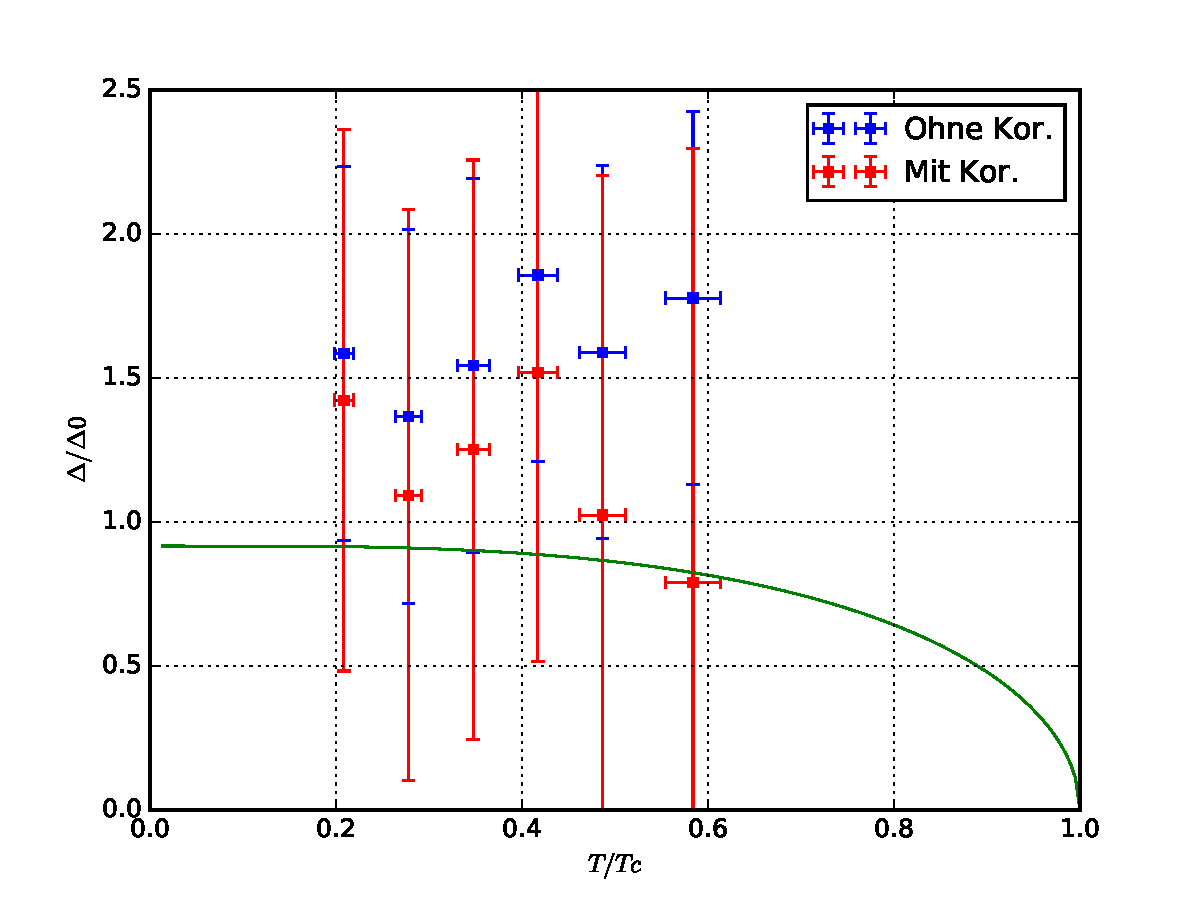
\includegraphics[scale=0.9]{4.pdf}
\caption{
In grün der theoretische Verlauf aus der BCS Therie nach Glg. (\ref{eq:korrun}), in blau die Werte ohne Korrektur, in rot die Werte nach Anwendung der Korrekturformel (\ref{eq:korrformel}).
Zudem liegt aufgrund der Achsenskalierung der BCS Wert für $T=0$ bei 1. 
In horizontal magenta ist auch der Literaturwert für Blei aus $\frac{2 \Delta_{Pb}}{k_{B} T_{C}} = 4.33 $ mit eingezeichnet. Es wird zudem dem klar, dass die BCS Theorie für Blei keinen guten Wert vorhersagt.
Auf den Grund wird in der Diskussion näher eingegangen.}
\label{fig:NLNL}
\end{figure}


\section{Diskussion}
Zunächst soll auf den Verlauf der Supraleiter-Normalleiter Kennlinie Abb. \ref{fig:SLNL} eingegangen werden.
Dabei zeigt sich wie schon aus Abb. \ref{fig:tunnel2} hervorgeht, bei höheren Temperaturen, dass die Messkurven stärker gekrümmt sind und 
sich nicht ein sehr flaches Plateau zeigt. 
Dies wird auch noch einmal durch die numerischen Ableitungen in Abb. \ref{eq:numdiff} der sechs Messreihen mit den in Tabelle \ref{tab:literatur} vermessenen Temperaturen deutlich.
Denn bei kleinen Temperaturen ist das Maximum der Ableitung eindeutiger.
Der dahinter stehende Grund wurde im Theorieteil kurz diskutiert, es findet nämlich eine Aufweichung der Fermikante statt, sodass manche Elektronen bereits bei geringerer Spannung die Barriere durchtunneln.

\begin{table}[]
\centering
\caption{Zum Vergleich der rel. Abw. zum lit wert $\frac{2 \Delta_{Pb}}{k_{B} T_{C}} = 4.33 \pm 0.1$ für Blei (PB)}
\label{my-label}
\begin{tabular}{|l|l|l|l|l|}
\hline
Temperatur K    & $\frac{2\Delta (T)}{k_{B} T_{C}}$ & Relative Abw. der unkorr. & $\frac{2\Delta_{K} (T)}{k_{B} T_{C}}$ & Relative Abw. der korr. \\ \hline
1.5 $\pm$ 0.075 & $3.5 \pm$ 0.14                    & 0.28                      & 5.0 $\pm$ 3.3                         & 0.15                    \\ \hline
2.0 $\pm$ 0.1   & 3.0 $\pm$ 0.14                    & 0.11                      & 3.8 $\pm$ 3.5                         & 0.11                    \\ \hline
2.5 $\pm$ 0.125 & 3.5 $\pm$ 0.14                    & 0.25                      & 4.4 $\pm$ 3.5                         & 0.02                    \\ \hline
3.0 $\pm$ 0.15  & 4.0$\pm$ 0.14                     & 0.50                      & 5.3 $\pm$ 3.5                         & 0.23                    \\ \hline
3.5 $\pm$ 0.175 & 3.5 $\pm$ 0.14                    & 0.29                      & 3.6 $\pm$ 4.1                         & 0.17                    \\ \hline
4.2 $\pm$ 0.21  & 3.9 $\pm$ 0.14                    & 0.44                      & 2.8 $\pm$ 5.3                         & 0.36                    \\ \hline
\end{tabular}
\label{tab:literatur}
\end{table}



Auch kann man erkennen, dass ab einem der Barriere entsprechenden Wert schließlich der Strom relativ sprunghaft einsetzt. 
Dies ist einleuchtend da nach Abb. \ref{fig:tunnel2} bei T=0 K die Steigung theoretisch sogar unendlich sein sollte.
Aber trotz verschiedener Temperaturen liegen alle Maxima (Abb. \ref{eq:numdiff}) mehr oder weniger im gleichen Spannungsintervall.
Dies rechtfertigt auch den recht groß gewählten Fehler von 1 mV, was der halben Breite einer Markierung auf der x-Achse entspricht. 
Durch diese Wahl sollten die "wahren" Maxima sehr wahrscheinlich im Fehlerintervall liegen.
An dieser Stelle soll aber noch einmal betont werden, dass selbstverständlich auch andere Methoden wie etwa Mittelwertbildung der Spannungskoordinaten um die Maxima mit einer höheren Gewichtung für Punkte in der Nähe des gemessenen absoluten Maximums eine Alternative gewesen wäre. 
Oder etwa auch das Bilden der zweiten numerischen Ableitung mit Nullstellensuche.
Da es aber kein unabhängiges Kriterium gibt zu prüfen ob diese Verfahren besserer gerechtfertigt sind haben wir uns für den erstgenannten Weg entschieden.
\\
Als Anmerkung sei noch erwähnt, das in die bereits genannten Abbildungen keine Fehlerbalken eingezeichnet wurden, da nur der eben diskutierte Fehler der Maxima entscheidend ist für die spätere Auswertung.
Zudem wären die Graphen dann aufgrund der Vielzahl an Punkten wesentlich unübersichtlicher.
\\
Um die Diskussion der Supraleiter-Normalleiter Kennlinie Abb. \ref{fig:SLNL} abzuschließen,
für große Spannungen nähern sich die Kennlinien dem (blauen) Verlauf, welcher Raumtemperatur entspricht,
nicht genau asymptotisch an, wie man es zunächst erwarten könnte, da bei hohen Energien die Cooperpaare aufgebrochen werden.
Der Grund ist, dass eine kleinere Steigung bei Messung der Raumtemperatur was einen größeren Widerstand bedeutet. Deshalb nähern sich die anderen Messreihen nicht genau asymptotisch an.
\\
Nachdem nun der qualitative Verlauf der Kennlinien besprochen wurde gilt es nun noch die Werte für die Energie Lücke oder auch charakteristische Anregungsenergie $\Delta$ im Hinblick auf Literaturwerte für Blei sowie der BCS Theorie einzuordnen.
Bei einer Temperatur von $T=1 K$ liegt der Literaturwert für Blei von 
$\frac{2 \Delta_{Pb}}{k_{B} T_{C}} = 4.33 \pm 0.1$ vor gemäß der Praktikumsanleitung.
Abschließend wird dieser Wert mit den im Experiment bestimmten Zahlen verglichen, siehe
Tabelle \ref{tab:literatur}.
Dabei sollte der entsprechende Wert bei $T=1 K$ diesem Literaturwert am nächsten kommen.
Dies ist zwar nicht der Fall, aber in der Tendenz ergibt sich eine kleinere Abweichung für niedrige Temperaturen in der Nähe von $1 K.$
\\
Die unkorrigierten Werte weichen im Mittel um 31 
\% die korrigierten um 17 \% ab.
Daher liegen die korrigierten Werte alle näher an der am Literaturwert für Blei. 
Die Korrekturformel (\ref{eq:korrformel}) liefert hier stets ausgehend von rechten Wert für das Spannungsmaximum
einen kleineren Wert für die Energielücke, indem berücksichtigt wird, dass bereits besetzte Zustände vorliegen. 
\\
Dies wird auch noch einmal durch Abb. \ref{fig:NLNL} deutlich.
Dort ist der Literaturwert für Blei als magentafarbene horizontale Linie neben dem Verlauf der BCS Theorie eingezeichnet.
Es wird hier auch ersichtlich, dass die Wahl der recht großen Fehler sich als gut erwiesen hat, da so alle Fehlerintervalle den Literaturwert schneiden.
\\
Nun noch der Vergleich mit der Kurve aus der BCS Theory, siehe dafür auch Abb. \ref{fig:NLNL}.
Auch hier ergeben sich durch die Korrektur bessere Ergebnisse für die Energielücke.
Um die Abweichung zwischen den korrigierten Werten und der BCS Kurve zu verdeutlichen wurde Abb. \ref{fig:comparison} erstellt. 
Dort zeigt sich mit Ausnahme eines Wertes bei 3 K, dass die Abweichung im Trend für größere Temperaturen kleiner wird. Um dies abschließend zu beurteilen würde man deutlich mehr Messwerte benötigen.
Dahingegen ist es eindeutig so, dass die BCS Theorie schon eindeutig durch den Vergleich des Literaturwertes für Blei mit der BCS Kurve in Abb. \ref{fig:NLNL} hier keine sehr genau Vorhersage liefert.
Der Grund ist mutmaßlich, dass die Bleiatome vergleichsweise schwer sind und daher eine starke
Elektron- Phonon-Kopplung vorliegt.
Die widerspricht aber einer Annahme der BCS Theorie wonach diese Wechselwirkung nur schwach
sein darf.
\\
Nun soll noch auf die Ursachen für die Abweichungen vom Literaturwert eingegangen werden.
Da wir wie Anfangs erwähnt die Daten eines anderes Versuch bekommen haben, können wir uns
bei den Temperaturen der Messung hinsichtlich des Fehlers nicht sicher sein.
Der Grund ist, dass wir nicht wissen bei welchen Temperaturen und bei welchem Druck der 
Dampfdruck des Helium erniedrigt wurde.
Hier haben wir uns einfach an den Fehlern eines Kommilitonen orientiert, da es sonst für uns keine Möglichkeit gab diesen einzuschätzen. 
\\
Sicher ist aber, dass sich der Druck während der Messung noch weiter verringert, sodass man 
die Temperatur über den gewünschten Wert hinaus erniedrigt. Hinzukommt noch der exponentielle
Zusammenhang der Dampfdruckkurve Abb. \ref{fig:dampf}, weshalb der Fehler mit steigender Temperatur
auch zunimmt.
\begin{figure}
\centering
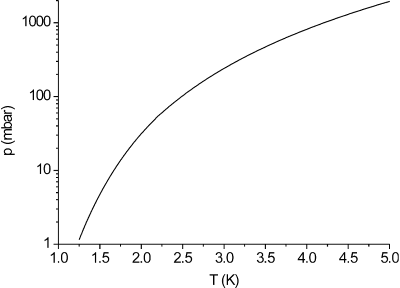
\includegraphics[scale=0.7]{Helium4Dampfgr.png}
\caption{Dampfdruckkurve von Helium 4,
Quelle: \url{http://www.pi1.uni-stuttgart.de/link/dampfdruck.html}}
\label{fig:dampf}
\end{figure}
\\
Zudem muss auch die Qualität der Probe und der Tunnelkontakte berücksichtigt werden.
Allerdings können wir wie schon erwähnt darüber keine Aussage treffen.
Klar ist aber, dass die Dicke der Oxidschicht einen starken Einfluss hat, weil diese die Tunnelbarriere darstellt.




 

\begin{figure}
\centering
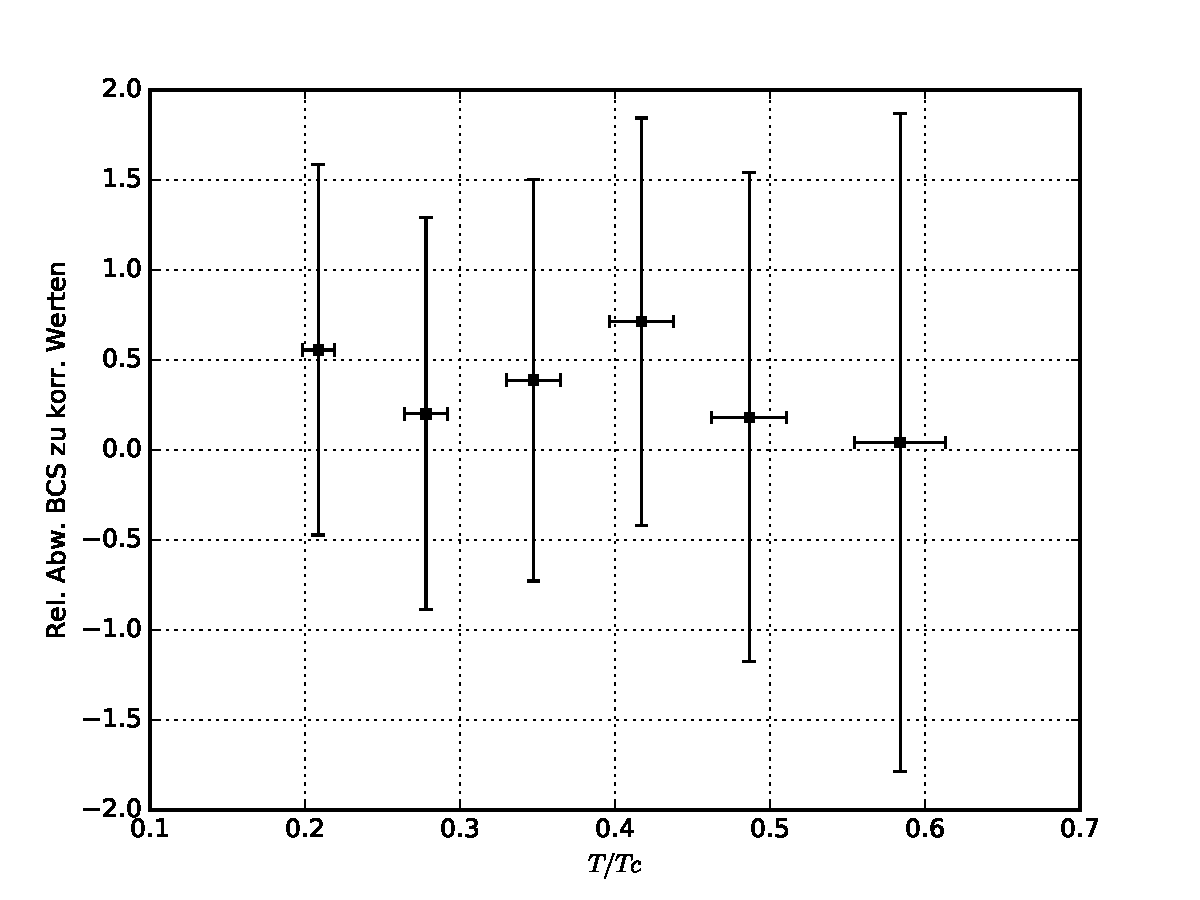
\includegraphics[scale=0.7]{5.pdf}
\caption{Gezeigt ist die relative Abweichung der korrigierten Werte aus der Messung zur BCS Theory Gleichung
 (\ref{eq:genauer})}
\label{fig:comparison}
\end{figure}





\section{Anhang}

\begin{figure}
\centering
\includegraphics[scale=0.15]{bild1.png}
\includegraphics[scale=0.15]{bild2.png}
\caption{
Oben: Aufdampfanlage und schon beschlagene Scheibe,
Unten: Kryostatversuchsanordnung
}
\label{fig:aufbau1}
\end{figure}

%\appendix
%
%\section{Anhang}
%
%
%\ldots
%
%\clearpage

% nicht unbedingt erforderlich
%\listoffigures
% nicht unbedingt erforderlich
%\listoftables

\bibliography{lit}

\end{document}